\chapter{Planificación} \label{ch:planificación}

\section{Metodología utilizada}

Para poder planificar este proyecto se ha optado por hacer uso de una de las metodologías ágiles mas utilizadas hoy en día, la metodología Scrum. Scrum es una metodología ágil para el desarrollo de software la gestión de proyectos. Antes de centrarnos en definir en que consiste aplicar una metodología Scrum es muy importante conocer que es una metodología ágil.

\subsection{Metodología Ágil}

La metodología ágil, más que una forma para llevar a cabo proyectos que requieren de rapidez y flexibilidad podría llegar a concebirse como una filosofía que presenta una forma distinta de trabajar y organizarse, adaptándose a las condiciones cambiantes que pueden surgir, aprovechando los cambios para obtener ventajas. Por medio de esta lo que se pretende es dividir un proyecto en pequeñas partes, de manera que este se realice de forma incremental o por fases, permitiendo así que dichas partes se pueden completar y entregarse lo mas rápido posible. 

Es importante tener en cuenta al definir la metodología ágil el propio manifiesto ágil \cite{manifiesto-agil}, que contiene los valores sobre los que se asientan dichos métodos y fuéron definidos en 2001. Estos valores son los siguientes:

\begin{itemize}
	\item Individuos e interacciones sobre procesos y herramientas
	\item Software funcionando sobre documentación extensiva
	\item Colaboración con el cliente sobre negociación contractual
	\item Respuesta ante el cambio sobre seguir un plan
\end{itemize}

Llevar a cabo una implementación ágil consta de 2 fases: análisis y realización de Sprint como se muestra en la Figura \ref{fig:metodologia-agil}.

\begin{figure}[h]
	\centering
	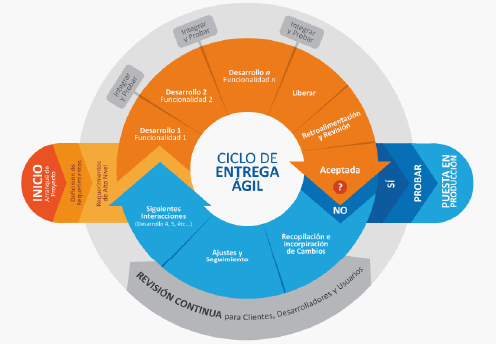
\includegraphics[width=1\textwidth]{img/metodologia-agil}
	\caption{Ciclo de entrega en proyectos ágiles.}
	\label{fig:metodologia-agil}
\end{figure}

A continución veremos en que consisten ambas fases:

\subsubsection{Fase 1: Análisis} \label{sssec:fase-analisis}
Esta fase consiste en 4 pasos:
\begin{enumerate}
	\item Preparación del proyecto durante el cual se definen los diferentes elementos, tales como labores,responsabilidades, estándares para la documentación y requisitos del hardware.
	\item Proceso de visualización en el que se identifican cuidadosamente todos los procesos operativos y procesos que dependen de condiciones específicas, como seguridad, autorizaciones e interfaces. Estos resultados serán la base para la construcción de unos cimientos sólidos para el proyecto entero.
	\item Funcionamiento de referencia del sistema, el cual se basará en el software de ERP.
	\item Fase de evaluación. En esta fase, se determina la prioridad de los requisitos adicionales y las funcionalidades, en orden del valor del negocio. Después de esto, el equipo de implementación estima el esfuerzo que será necesario para realizar esto y determina la planificación de los Sprints para que se suministren los componentes del sistema.
\end{enumerate}

\subsubsection{Fase 2: Realización del Sprint}

Esta fase consiste en 5 pasos:

\begin{enumerate}
	\item Reuniones de planificación al comienzo de cada Sprint. Se define el objetivo del Sprint entre el propietario y el equipo de implementación.
	\item Realización de los requisitos, de pruebas y documentación.
	\item Reuniones diarias del estado del proyecto. En esta fase se registra el estado del proyecto y se discuten los diversos obstáculos que el equipo ha podido encontrar.
	\item Sesión de prueba del Sprint. Durante esta fase los usuarios y el equipo IT determinan si los procesos cumplen los requisitos.
	\item Se llevará a cabo una revisión del Sprint para comprobar que se puede mejorar en los futuros Sprints.
\end{enumerate}

\subsection{Metodología Scrum}

Como hemos dicho al inicio de este capítulo, Scrum es una metodología ágil para el desarrollo de software o la gestión de proyectos, más específicamente, es un marco de trabajo a través del cual las personas pueden abordar problemas complejos adaptativos, mientras que se entregan productos de forma eficiente y creativa con el máximo valor \cite{scrum-guia}.

Scrum está compuesto por diferentes procesos que se utilizan para la gestión del trabajo de producto complejos desde inicios de los años 90. Como tal, Scrum no es un proceso, una técnica o un método definitivo, es un marco de trabajo donde se puede emplear un conjunto de diversos procesos o técnicas. Scrum muestra la eficacia relativa de las técnicas de gestión de producto y de trabajo de modo que podamos mejorar de forma continua el producto, equipo y entorno de trabajo. El marco de trabajo de Scrum está compuesto por los Equipos Scrum, sus Roles, Eventos, Artefactos y Reglas asociadas. Cada uno de ellos sirve a un propósito específico y de la misma forma es esencial para el éxito de Scrum y para su uso.

En un principio, Scrum fue desarrollado para gestionar y desarrollar productos. Con el tiempo, y más a partir de 1990, se ha llegado a utilizar en diferentes ámbitos: desarrollo de software, hardware, redes funcionales, vehículos autónomos, escuelas, gobiernos, marketing y en la totalidad de todo lo que hacemos uso en nuestra vida, tanto como individuos y sociedad.

La esencia de Scrum reside en trabajar en pequeños equipos, siendo estos individualmente flexibles y adaptativos. Estas características siguen manteniéndose tanto en equipos individuales, varios, muchos u redes que equipos encargados de desarrollar, lanzar, operar y mantener el trabajo y el producto. Entre los diferentes equipos colaboran e ínter-operan a través del desarrollo de sofisticadas arquitecturas y objetivos en entornos de desarrollo.

\subsubsection{Características de Scrum}

Entre todas las metodologías ágiles, Scrum se basa en la teoría de control empírica de los procesos. Esto significa que se utiliza el progreso real de un proceso para poder planificar y concretar los lanzamientos. Scrum trabaja de forma que los proyectos están divididos en Sprints, los cuales tienen una duración de entre dos a cuatro semanas. Cuando finaliza un Sprint, se realiza una reunión entres los miembros del equipo y el cliente con el fin de mostrar al cliente el proyecto y que este pueda ser evaluado de cara a poder planificar las tareas que se deberán de utilizar en el siguiente Sprint como se ve en la Figura \ref{fig:scrum}. Con esto lo que se pretende es que la dirección del proyecto pueda ajustarse o reorientarse una vez haya finalizado y durante el mismo mantener un control de los riesgos.

\begin{figure}[h]
	\centering
	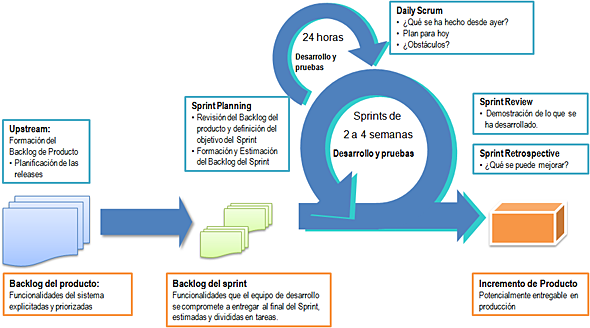
\includegraphics[width=1\textwidth]{img/scrum}
	\caption{Ciclo de vida de Scrum.}
	\label{fig:scrum}
\end{figure}

\newpage
Existen tres pilares sobre los que se fundamentará el control empírico de Scrum:

\begin{enumerate}
	\item \textbf{Transparencia:} Los aspectos significativos han de ser visibles para todos aquellos responsables del resultado.
	\item \textbf{Inspección:} Se han de inspeccionar frecuentemente los artefactos y el progreso hacia el objetivo, para detectar variaciones.
	\item \textbf{Adaptación:}  Capacidad para adaptarse en el caso de que el proceso se desvíe de los límites aceptables.
\end{enumerate}

\subsubsection{Roles de Scrum}

Un equipo de \textbf{Scrum} suele estar formados por unos pocos miembros, entre 3 y 9, sin incluir al Scrum Manager y el Product Owner. Cada uno de ellos tiene por tanto diferentes roles y responsabilidades dentro del proyecto. Procederemos a continuación a explicar las diferentes responsabilidades de cada uno de ellos

\begin{itemize}
	\item \textbf{Product Owner}: Es el rol principal del proyecto. Suele ser el encargado de representar al cliente o ser directamente el propio cliente. ha de preservar los intereses del cliente priorizando las diferentes tareas para alcanzar los objetivos propuestos y establecer los diferentes requisitos del proyecto. De los tres roles, es el que mayor responsabilidades tiene, por lo que si algo no funciona o sale mal la responsabilidad recae sobre el. Para que el Product Owner pueda hacer bien su trabajo, todos han de respetar sus decisiones. A su vez el Product Owner debería evitar la supervisión de cada detalle del proyecto, pero sin embargo ha de estar disponible en caso de que el equipo de desarrollo tenga alguna pregunta o duda.
	\item \textbf{Scrum Master}: Es el rol encargado de actuar como enlace entre el Product Owner y el equipo de desarrollo. Como tal el Scrum Master ha de encargarse de resolver los diferentes conflictos que puedan obstaculizar el ritmo del proyecto. Este a su vez ha de incentivar u motivar al equipo de desarrollo para poder hacer visibles los logros del mismo ante del Product Owner. De cara al Product Owner, el Scrum Master le ofrecerá el apoyo necesario para poder maximizar los resultados.
	\item \textbf{Equipo de desarrollo}: Es el rol que se le da al conjunto del equipo que trabaja en el equipo, el cual será el encargado de terminar el trabajo. Estos equipos han de ser auto-organizados, multifuncionales, aunque cada miembro del equipo puede tener habilidades especializadas en un área, aunque la responsabilidad recae sobre el equipo y no sobre el individuo. A su vez, no se reconocen títulos dentro del equipo, independientemente del trabajo que realicen sus miembros así como tampoco se reconocen  los sub-equipo, independientemente de los dominios sobre los que se trabajen
\end{itemize}

\begin{figure}[H]
	\centering
	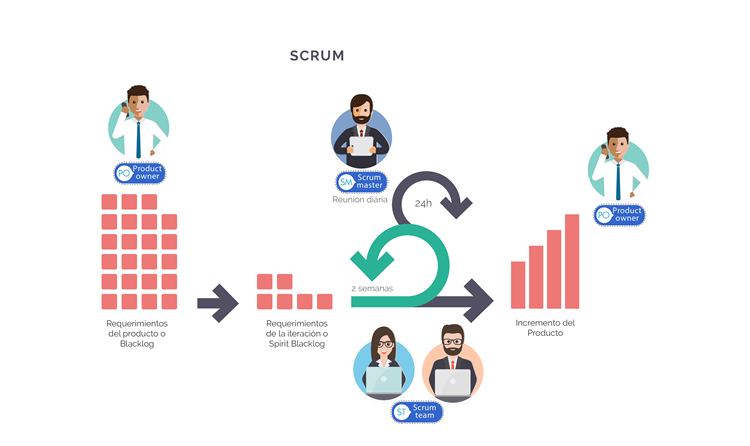
\includegraphics[width=1\textwidth]{img/roles-scrum}
	\caption{Estructura de la participación de los roles en el Scrum.}
	\label{fig:roles-scrum}
\end{figure}

\section{Historias de usuario y tareas} \label{sec:historias-tareas}

En este punto se tiene que ser capaz de plantear los objetivos que han de ser alcanzados a lo largo del desarrollo del producto final. Para hacer esto se hará uso de una serie de \textbf{Historias de Usuarios}, un elemento básico a la hora de aplicar metodologías ágiles en un proyecto y especialmente para poder aplicar \textbf{Scrum}. Las \textbf{Historias de Usuario} representarán de manera breve las características demandadas por el cliente las cuales deberán formar parte de la funcionalidad del producto, satisfaciendo sus exigencias.

El proceso por el cual se realiza la extracción de información relacionada con la funcionalidad del proyecto se debe llevar a cabo entre los miembros del equipo y el propio cliente. Al aplicar \textbf{Scrum}, este proceso no solo se realizará en la fase inicial del proyecto, si no que se realizan en cada Sprint del proyecto, de manera que se pueda obtener el resultado esperado en un corto espacio de tiempo y permitiendo amoldar el proyecto a lo requerido por el cliente de la forma mas eficiente posible.

Las \textbf{Historias de Usuario}, en términos generales, siempre han de extraerse durante las reuniones con el cliente y es deseable que sean escritas por el mismo y en un lenguaje claro, sin entrar en detalles. Estas han de aportarnos la funcionalidad requerida por el proyecto, entregando de esta forma un valor particular al cliente.

Estas han de desglosarse en tres apartados:

\begin{itemize}
	\item \textbf{Como}: representa el rol que va a utilizar el proyecto
	\item \textbf{Quiere}: representa la acción o evento que quiere que ocurra
	\item \textbf{Para}: representa la funcionalidad que se quiere cubrir.
\end{itemize}

A su vez tambien puede usarse la estructura presentada por la web Scrum Manager \cite{scrum-manager}:

\begin{itemize}
	\item Nombre breve y descriptivo.
	\item Descripción de la funcionalidad en forma de diálogo o monólogo del usuario describiendo la funcionalidad que desea realizar.
	\item Criterio de validación y verificación que determinará para considerar terminado y aceptable por el cliente el desarrollo de la funcionalidad descrita.
\end{itemize}

Como se ha dicho antes, las \textbf{Historias de Usuario} ayudan a modelar el producto según las necesidades del cliente y mediante una reunión entre el equipo y este. El cliente aportará la idea que tiene, las necesidades que pretende cubrir y las funcionalidades que en cada momento el estima oportunas para el proyecto. A su vez, el equipo encargado del desarrollo también podrán aportar su punto de vista en ciertos puntos con la finalidad de poder enriquecer el proyecto. Para finalizar el Product Owner, que actúa como la voz del cliente dentro del equipo, será el encargado de redactar las \textbf{Historias de Usuario} y de extraer las diferentes tareas resultantes de las mismas, identificándolas según el coste su coste y prioridad. Con esto lo que se consigue es definir el Product Backlog, base a la hora de aplicar Scrum a un proyecto.

Es importante recalcar que en el Product Backlog se indicaran los diferentes Sprints del proyecto y las tareas asociadas a los mismos. Esto no quiere decir que se mantenga durante todo el proyecto, pues la definición obtenida al inicio del mismo puede varias dependiendo de las necesidades del cliente. Dado que el proyecto estará dividido en una serie de Sprints, durante los mismos debería realizarse una reunión entre los diferentes miembros del equipo y el cliente donde se podrán hacer adaptaciones que se consideren convenientes permitiendo cambiar o replantear los objetivos del proyecto con el fin de maximizar su utilidad.

Las \textbf{Historias de Usuario} serán definidas con la siguiente estructura:

\rowcolors{1}{gray!30}{gray!10}
\begin{table}[H]
	\begin{center}
		\begin{tabular}{| c | p{9cm} |}
			\hline
			
			Historia de Usuario &  \\ \hline
			
			
			\textbf{ID} & HUXX \\
			\textbf{Nombre} &  \\
			\textbf{Prioridad} &  \\
			\textbf{Riesgo} &  \\
			\textbf{Descripción} &  \\
			\textbf{Validación} &  \\ \hline
		\end{tabular}
		\caption{Modelo Historia de Usuario.}
	\end{center}
\end{table}

Cada campo de las \textbf{Historias de Usuario} representa lo siguiente:

\begin{itemize}
	\item \textbf{ID}: Identificar único de la Historia de Usuario.
	\item \textbf{Nombre}: Nombre asignado a la Historia de Usuario
	\item \textbf{Prioridad}: Importancia a la hora de llevar a cabo en el desarrollo, pudiendo ser alta, media o baja
	\item \textbf{Riesgo}: Importancia en relación al conjunto del proyecto, indicando así en caso de fallo el daño provocado, pudiendo ser alto, medio o bajo. .
	\item \textbf{Descripción}: Explicación de la Historia de Usuario, dejando clara la idea de la misma
	\item \textbf{Validación}: Condiciones que se han de cumplir para dar la historia por finalizada.
\end{itemize}

\subsection{Historias de Usuario}

Las \textbf{Historias de Usuario} que se han creado para este proyecto son las siguientes:

\rowcolors{1}{gray!30}{gray!10}
\begin{table}[H]
	\begin{center}
		\begin{tabular}{| c | p{9cm} |}
			\hline
			
			Historia de Usuario &  \\ \hline
			
			
			\textbf{ID} & HU01 \\
			\textbf{Nombre} & Apariencia \\
			\textbf{Prioridad} & Media \\
			\textbf{Riesgo} & Baja \\
			\textbf{Descripción} & Como usuario quiero que el bot tenga un diseño simple, sencillo e intuitivo. \\
			\textbf{Validación} & \begin{itemize}
				\item Quiero acceder a la información pulsando un botón.
				\item Quiero ver todos los datos de manera clara.
				\item Todos los botones han de tener un funcionamiento claro.
			\end{itemize} \\ \hline
		\end{tabular}
		\caption{Historia de Usuario - Apariencia.}
	\end{center}
\end{table}

\begin{table}[H]
	\begin{center}
		\begin{tabular}{| c | p{9cm} |}
			\hline
			
			Historia de Usuario &  \\ \hline
			
			
			\textbf{ID} & HU02 \\
			\textbf{Nombre} & Funcionamiento \\
			\textbf{Prioridad} & Media \\
			\textbf{Riesgo} & Baja \\
			\textbf{Descripción} & Como usuario quiero poder hacer uso del Bot en todo momento, principalmente en un dispositivo móvil, para poder consultar información en cualquier lugar. \\
			\textbf{Validación} & \begin{itemize}
				\item Quiero que el Bot funcione sobre todo en móviles.
				\item Quiero que tenga un acceso fácil.
			\end{itemize} \\ \hline
		\end{tabular}
		\caption{Historia de Usuario - Funcionamiento.}
	\end{center}
\end{table}

\begin{table}[H]
	\begin{center}
		\begin{tabular}{| c | p{9cm} |}
			\hline
			
			Historia de Usuario &  \\ \hline
			
			
			\textbf{ID} & HU03 \\
			\textbf{Nombre} & Menú Principal \\
			\textbf{Prioridad} & Alta \\
			\textbf{Riesgo} & Baja \\
			\textbf{Descripción} & Como usuario quiero tener un menú principal que se muestre en todo momento y me permita acceder a las diferentes utilidades del Bot. \\
			\textbf{Validación} & \begin{itemize}
				\item Quiero que el menú se muestre siempre por defecto salvo que el usuario decida ocultarlo.
				\item Quiero poder acceder al menú principal del Bot.
				\item Quiero poder acceder a la ayuda del Bot.
				\item Quiero poder acceder a la información de desarrollo del Bot.
			\end{itemize} \\ \hline
		\end{tabular}
		\caption{Historia de Usuario - Menú Principal.}
	\end{center}
\end{table}

\begin{table}[H]
	\begin{center}
		\begin{tabular}{| c | p{9cm} |}
			\hline
			
			Historia de Usuario &  \\ \hline
			
			
			\textbf{ID} & HU04 \\
			\textbf{Nombre} & Seleccionar Comunidad Autónoma \\
			\textbf{Prioridad} & Alta \\
			\textbf{Riesgo} & Baja \\
			\textbf{Descripción} & Como usuario quiero poder seccionar la provincia de la que quiero consultar los datos. \\
			\textbf{Validación} & \begin{itemize}
				\item Quiero poder seleccionar entre todas las CCAA del territorio español.
				\item Quiero poder seleccionar toda España.
				\item Las CCAA deben verse todas a la vez en pantalla.
				\item Las CCAA han de mostrarse de manera clara y ordenada.
			\end{itemize} \\ \hline
		\end{tabular}
		\caption{Historia de Usuario - Selección Comunidad Autónoma.}
	\end{center}
\end{table}

\begin{table}[H]
	\begin{center}
		\begin{tabular}{| c | p{9cm} |}
			\hline
			
			Historia de Usuario &  \\ \hline
			
			
			\textbf{ID} & HU05 \\
			\textbf{Nombre} & Seleccionar datos \\
			\textbf{Prioridad} & Alta \\
			\textbf{Riesgo} & Media \\
			\textbf{Descripción} & Como usuario quiero poder seccionar los datos que quiero consultar. \\
			\textbf{Validación} & \begin{itemize}
				\item Los datos han de mostrarse en diferentes apartados.
				\item Pueden consultarse los datos mas actuales.
				\item Pueden consultase los datos desde el inicio de la pandemia.
				\item En algunos datos deben mostrarse gráficas (mostrar evolución de manera clara).
				\item Poder consultar la acumulación de casos.
				\item Poder ver el nº de fallecidos.
				\item Poder ver el nº de hospitalizados.
				\item Poder ver una lista de las provincias con más casos (solo al consultar España)
				\item Poder ver las incidencias actuales por cada 100k habitantes por provincias (solo al consultar España)
				\item Poder ver las incidencias desde el inicio de la pandemia por cada 100k habitantes por provincias (solo al consultar España)
				\item Poder ver como afecta el virus dependiendo de la edad (solo al consultar España)
			\end{itemize} \\ \hline
		\end{tabular}
		\caption{Historia de Usuario - Selección datos.}
	\end{center}
\end{table}

\begin{table}[H]
	\begin{center}
		\begin{tabular}{| c | p{9cm} |}
			\hline
			
			Historia de Usuario &  \\ \hline
			
			
			\textbf{ID} & HU06 \\
			\textbf{Nombre} & Seleccionar ayuda \\
			\textbf{Prioridad} & Alta \\
			\textbf{Riesgo} & Baja \\
			\textbf{Descripción} & Como usuario quiero poder acceder a una opción en todo momento por si tengo alguna duda. \\
			\textbf{Validación} & \begin{itemize}
				\item Esta opción ha de mostrarse en todo momento salvo que el usuario la oculte.
				\item Esta opción ha de estar en el menú principal.
				\item Quiero poder ver que es cada uno de los apartados del proyecto.
			\end{itemize} \\ \hline
		\end{tabular}
		\caption{Historia de Usuario - Selección ayuda.}
	\end{center}
\end{table}

\begin{table}[H]
	\begin{center}
		\begin{tabular}{| c | p{9cm} |}
			\hline
			
			Historia de Usuario &  \\ \hline
			
			
			\textbf{ID} & HU07 \\
			\textbf{Nombre} & Seleccionar información \\
			\textbf{Prioridad} & Alta \\
			\textbf{Riesgo} & Baja \\
			\textbf{Descripción} & Como desarrollador quiero que el usuario pueda consultar datos sobre el proyecto. \\
			\textbf{Validación} & \begin{itemize}
				\item Esta opción ha de mostrarse en todo momento salvo que el usuario la oculte.
				\item Esta opción ha de estar en el menú principal.
				\item Quiero mostrar al usuario la información principal del desarrollo del proyecto.
			\end{itemize} \\ \hline
		\end{tabular}
		\caption{Historia de Usuario - Selección información.}
	\end{center}
\end{table}

\begin{table}[H]
	\begin{center}
		\begin{tabular}{| c | p{9cm} |}
			\hline
			
			Historia de Usuario &  \\ \hline
			
			
			\textbf{ID} & HU08 \\
			\textbf{Nombre} & Despliegue \\
			\textbf{Prioridad} & Alta \\
			\textbf{Riesgo} & Baja \\
			\textbf{Descripción} & Como desarrollador quiero que el Bot funcione en todo momento. \\
			\textbf{Validación} & \begin{itemize}
				\item El Bot y sus datos han de estar en un contenedor.
				\item El Bot ha de desplegarse como un PaaS.
			\end{itemize} \\ \hline
		\end{tabular}
		\caption{Historia de Usuario - Despliegue.}
	\end{center}
\end{table}

\begin{table}[H]
	\begin{center}
		\begin{tabular}{| c | p{9cm} |}
			\hline
			
			Historia de Usuario &  \\ \hline
			
			
			\textbf{ID} & HU09 \\
			\textbf{Nombre} & Modularización \\
			\textbf{Prioridad} & Alta \\
			\textbf{Riesgo} & Baja \\
			\textbf{Descripción} & Como programador, quiero modularizar algunas partes de forma que sean fáciles de manejar y testear. \\
			\textbf{Validación} & \begin{itemize}
				\item Quiero de los diferentes módulos puedan pasar los test.
				\item Quiero que el código esté dividido por funcionalidad.
			\end{itemize} \\ \hline
		\end{tabular}
		\caption{Historia de Usuario - Modularización.}
	\end{center}
\end{table}

\newpage
\subsection{Tareas}

A su vez, las \textbf{Historias de Usuario} estarán divididos en una serie de \textbf{Tareas}. Las \textbf{Tareas} serán definidas con la siguiente estructura:

\begin{table}[H]
	\begin{center}
		\begin{tabular}{| c | p{9cm} |}
			\hline
			
			\textbf{Tarea} & TXX \\
			\textbf{Historia de Usuario} &  \\
			\textbf{Estado} &  \\
			\textbf{Descripción} &  \\ \hline
		\end{tabular}
		\caption{Modelo Tarea.}
	\end{center}
\end{table}

Cada campo de las \textbf{Historias de Usuario} representa lo siguiente:

\begin{itemize}
	\item \textbf{Tarea}: Identificar único de la Tarea.
	\item \textbf{Historia de Usuario}: Historia de Usuario a la que está asociada la Tarea
	\item \textbf{Estado}: Fase en la que se encuentra la Tarea dentro del proyecto, pudiendo ser No iniciada, En proceso o Completada
	\item \textbf{Descripción}: Explicación de la Historia de Usuario, dejando clara la idea de la misma
\end{itemize}

Las \textbf{Tareas} que se han creado para este proyecto son las siguientes:

\begin{table}[H]
	\begin{center}
		\begin{tabular}{| c | p{9cm} |}
			\hline
			
			\textbf{Tarea} & T01 \\
			\textbf{Historia de Usuario} & HU02 \\
			\textbf{Estado} & Completada \\
			\textbf{Descripción} & Seleccionar la plataforma donde vamos a desarrollar el Bot \\ \hline
		\end{tabular}
		\caption{Tarea 01.}
	\end{center}
\end{table}

\begin{table}[H]
	\begin{center}
		\begin{tabular}{| c | p{9cm} |}
			\hline
			
			\textbf{Tarea} & T02 \\
			\textbf{Historia de Usuario} & HU01 \\
			\textbf{Estado} & Completada \\
			\textbf{Descripción} & Crear la disposición y diseño de botones del Menú principal \\ \hline
		\end{tabular}
		\caption{Tarea 02.}
	\end{center}
\end{table}

\begin{table}[H]
	\begin{center}
		\begin{tabular}{| c | p{9cm} |}
			\hline
			
			\textbf{Tarea} & T03 \\
			\textbf{Historia de Usuario} & HU01 \\
			\textbf{Estado} & Completada \\
			\textbf{Descripción} & Crear la disposición y diseño de botones del Menú de selección de comunidades \\ \hline
		\end{tabular}
		\caption{Tarea 03.}
	\end{center}
\end{table}

\begin{table}[H]
	\begin{center}
		\begin{tabular}{| c | p{9cm} |}
			\hline
			
			\textbf{Tarea} & T04 \\
			\textbf{Historia de Usuario} & HU01 \\
			\textbf{Estado} & Completada \\
			\textbf{Descripción} & Crear la disposición y diseño de botones del Menú de información a consultar de cada comunidad en sus diferentes estados \\ \hline
		\end{tabular}
		\caption{Tarea 04.}
	\end{center}
\end{table}

\begin{table}[H]
	\begin{center}
		\begin{tabular}{| c | p{9cm} |}
			\hline
			
			\textbf{Tarea} & T05 \\
			\textbf{Historia de Usuario} & HU01 \\
			\textbf{Estado} & Completada \\
			\textbf{Descripción} & Crear la disposición y diseño de botones del Menú de información a consultar de España en sus diferentes estados \\ \hline
		\end{tabular}
		\caption{Tarea 05.}
	\end{center}
\end{table}

\begin{table}[H]
	\begin{center}
		\begin{tabular}{| c | p{9cm} |}
			\hline
			
			\textbf{Tarea} & T06 \\
			\textbf{Historia de Usuario} & HU03 \\
			\textbf{Estado} & Completada \\
			\textbf{Descripción} & Crear el Menú principal y configurarlo para que sea visible en todo momento salvo que el usuario decida ocultarlo \\ \hline
		\end{tabular}
		\caption{Tarea 06.}
	\end{center}
\end{table}

\begin{table}[H]
	\begin{center}
		\begin{tabular}{| c | p{9cm} |}
			\hline
			
			\textbf{Tarea} & T07 \\
			\textbf{Historia de Usuario} & HU03 \\
			\textbf{Estado} & Completada \\
			\textbf{Descripción} & Implementar la funcionalidad del botón Menú para acceder al listado de comunidades \\ \hline
		\end{tabular}
		\caption{Tarea 07.}
	\end{center}
\end{table}

\begin{table}[H]
	\begin{center}
		\begin{tabular}{| c | p{9cm} |}
			\hline
			
			\textbf{Tarea} & T08 \\
			\textbf{Historia de Usuario} & HU03 \\
			\textbf{Estado} & Completada \\
			\textbf{Descripción} & Implementar la funcionalidad del botón Ayuda \\ \hline
		\end{tabular}
		\caption{Tarea 08.}
	\end{center}
\end{table}

\begin{table}[H]
	\begin{center}
		\begin{tabular}{| c | p{9cm} |}
			\hline
			
			\textbf{Tarea} & T09 \\
			\textbf{Historia de Usuario} & HU03 \\
			\textbf{Estado} & Completada \\
			\textbf{Descripción} & Implementar la funcionalidad del botón Información \\ \hline
		\end{tabular}
		\caption{Tarea 09.}
	\end{center}
\end{table}

\begin{table}[H]
	\begin{center}
		\begin{tabular}{| c | p{9cm} |}
			\hline
			
			\textbf{Tarea} & T10 \\
			\textbf{Historia de Usuario} & HU04 \\
			\textbf{Estado} & Completada \\
			\textbf{Descripción} & Crear el Menú de comunidades y España \\ \hline
		\end{tabular}
		\caption{Tarea 10.}
	\end{center}
\end{table}

\begin{table}[H]
	\begin{center}
		\begin{tabular}{| c | p{9cm} |}
			\hline
			
			\textbf{Tarea} & T11 \\
			\textbf{Historia de Usuario} & HU05 \\
			\textbf{Estado} & Completada \\
			\textbf{Descripción} & Implementar la funcionalidad de los botones de consulta de datos para Andalucía \\ \hline
		\end{tabular}
		\caption{Tarea 11.}
	\end{center}
\end{table}

\begin{table}[H]
	\begin{center}
		\begin{tabular}{| c | p{9cm} |}
			\hline
			
			\textbf{Tarea} & T12 \\
			\textbf{Historia de Usuario} & HU05 \\
			\textbf{Estado} & Completada \\
			\textbf{Descripción} & Implementar la funcionalidad de los botones de consulta de datos para Aragón \\ \hline
		\end{tabular}
		\caption{Tarea 12.}
	\end{center}
\end{table}

\begin{table}[H]
	\begin{center}
		\begin{tabular}{| c | p{9cm} |}
			\hline
			
			\textbf{Tarea} & T13 \\
			\textbf{Historia de Usuario} & HU05 \\
			\textbf{Estado} & Completada \\
			\textbf{Descripción} & Implementar la funcionalidad de los botones de consulta de datos para Asturias \\ \hline
		\end{tabular}
		\caption{Tarea 13.}
	\end{center}
\end{table}

\begin{table}[H]
	\begin{center}
		\begin{tabular}{| c | p{9cm} |}
			\hline
			
			\textbf{Tarea} & T14 \\
			\textbf{Historia de Usuario} & HU05 \\
			\textbf{Estado} & Completada \\
			\textbf{Descripción} & Implementar la funcionalidad de los botones de consulta de datos para C. Valenciana \\ \hline
		\end{tabular}
		\caption{Tarea 14.}
	\end{center}
\end{table}

\begin{table}[H]
	\begin{center}
		\begin{tabular}{| c | p{9cm} |}
			\hline
			
			\textbf{Tarea} & T15 \\
			\textbf{Historia de Usuario} & HU05 \\
			\textbf{Estado} & Completada \\
			\textbf{Descripción} & Implementar la funcionalidad de los botones de consulta de datos para Canarias \\ \hline
		\end{tabular}
		\caption{Tarea 15.}
	\end{center}
\end{table}

\begin{table}[H]
	\begin{center}
		\begin{tabular}{| c | p{9cm} |}
			\hline
			
			\textbf{Tarea} & T16 \\
			\textbf{Historia de Usuario} & HU05 \\
			\textbf{Estado} & Completada \\
			\textbf{Descripción} & Implementar la funcionalidad de los botones de consulta de datos para Cantabria \\ \hline
		\end{tabular}
		\caption{Tarea 16.}
	\end{center}
\end{table}

\begin{table}[H]
	\begin{center}
		\begin{tabular}{| c | p{9cm} |}
			\hline
			
			\textbf{Tarea} & T17 \\
			\textbf{Historia de Usuario} & HU05 \\
			\textbf{Estado} & Completada \\
			\textbf{Descripción} & Implementar la funcionalidad de los botones de consulta de datos para Castilla La Mancha \\ \hline
		\end{tabular}
		\caption{Tarea 17.}
	\end{center}
\end{table}

\begin{table}[H]
	\begin{center}
		\begin{tabular}{| c | p{9cm} |}
			\hline
			
			\textbf{Tarea} & T18 \\
			\textbf{Historia de Usuario} & HU05 \\
			\textbf{Estado} & Completada \\
			\textbf{Descripción} & Implementar la funcionalidad de los botones de consulta de datos para Castilla y León \\ \hline
		\end{tabular}
		\caption{Tarea 18.}
	\end{center}
\end{table}

\begin{table}[H]
	\begin{center}
		\begin{tabular}{| c | p{9cm} |}
			\hline
			
			\textbf{Tarea} & T19 \\
			\textbf{Historia de Usuario} & HU05 \\
			\textbf{Estado} & Completada \\
			\textbf{Descripción} & Implementar la funcionalidad de los botones de consulta de datos para Cataluña \\ \hline
		\end{tabular}
		\caption{Tarea 19.}
	\end{center}
\end{table}

\begin{table}[H]
	\begin{center}
		\begin{tabular}{| c | p{9cm} |}
			\hline
			
			\textbf{Tarea} & T20 \\
			\textbf{Historia de Usuario} & HU05 \\
			\textbf{Estado} & Completada \\
			\textbf{Descripción} & Implementar la funcionalidad de los botones de consulta de datos para Ceuta \\ \hline
		\end{tabular}
		\caption{Tarea 20.}
	\end{center}
\end{table}

\begin{table}[H]
	\begin{center}
		\begin{tabular}{| c | p{9cm} |}
			\hline
			
			\textbf{Tarea} & T21 \\
			\textbf{Historia de Usuario} & HU05 \\
			\textbf{Estado} & Completada \\
			\textbf{Descripción} & Implementar la funcionalidad de los botones de consulta de datos para Extremadura \\ \hline
		\end{tabular}
		\caption{Tarea 21.}
	\end{center}
\end{table}

\begin{table}[H]
	\begin{center}
		\begin{tabular}{| c | p{9cm} |}
			\hline
			
			\textbf{Tarea} & T22 \\
			\textbf{Historia de Usuario} & HU05 \\
			\textbf{Estado} & Completada \\
			\textbf{Descripción} & Implementar la funcionalidad de los botones de consulta de datos para Galicia \\ \hline
		\end{tabular}
		\caption{Tarea 22.}
	\end{center}
\end{table}

\begin{table}[H]
	\begin{center}
		\begin{tabular}{| c | p{9cm} |}
			\hline
			
			\textbf{Tarea} & T23 \\
			\textbf{Historia de Usuario} & HU05 \\
			\textbf{Estado} & Completada \\
			\textbf{Descripción} & Implementar la funcionalidad de los botones de consulta de datos para Baleares \\ \hline
		\end{tabular}
		\caption{Tarea 23.}
	\end{center}
\end{table}

\begin{table}[H]
	\begin{center}
		\begin{tabular}{| c | p{9cm} |}
			\hline
			
			\textbf{Tarea} & T24 \\
			\textbf{Historia de Usuario} & HU05 \\
			\textbf{Estado} & Completada \\
			\textbf{Descripción} & Implementar la funcionalidad de los botones de consulta de datos para La Rioja \\ \hline
		\end{tabular}
		\caption{Tarea 24.}
	\end{center}
\end{table}

\begin{table}[H]
	\begin{center}
		\begin{tabular}{| c | p{9cm} |}
			\hline
			
			\textbf{Tarea} & T25 \\
			\textbf{Historia de Usuario} & HU05 \\
			\textbf{Estado} & Completada \\
			\textbf{Descripción} & Implementar la funcionalidad de los botones de consulta de datos para Madrid \\ \hline
		\end{tabular}
		\caption{Tarea 25.}
	\end{center}
\end{table}

\begin{table}[H]
	\begin{center}
		\begin{tabular}{| c | p{9cm} |}
			\hline
			
			\textbf{Tarea} & T26 \\
			\textbf{Historia de Usuario} & HU05 \\
			\textbf{Estado} & Completada \\
			\textbf{Descripción} & Implementar la funcionalidad de los botones de consulta de datos para Melilla \\ \hline
		\end{tabular}
		\caption{Tarea 26.}
	\end{center}
\end{table}

\begin{table}[H]
	\begin{center}
		\begin{tabular}{| c | p{9cm} |}
			\hline
			
			\textbf{Tarea} & T27 \\
			\textbf{Historia de Usuario} & HU05 \\
			\textbf{Estado} & Completada \\
			\textbf{Descripción} & Implementar la funcionalidad de los botones de consulta de datos para Murcia \\ \hline
		\end{tabular}
		\caption{Tarea 27.}
	\end{center}
\end{table}

\begin{table}[H]
	\begin{center}
		\begin{tabular}{| c | p{9cm} |}
			\hline
			
			\textbf{Tarea} & T28 \\
			\textbf{Historia de Usuario} & HU05 \\
			\textbf{Estado} & Completada \\
			\textbf{Descripción} & Implementar la funcionalidad de los botones de consulta de datos para Navarra \\ \hline
		\end{tabular}
		\caption{Tarea 28.}
	\end{center}
\end{table}

\begin{table}[H]
	\begin{center}
		\begin{tabular}{| c | p{9cm} |}
			\hline
			
			\textbf{Tarea} & T29 \\
			\textbf{Historia de Usuario} & HU05 \\
			\textbf{Estado} & Completada \\
			\textbf{Descripción} & Implementar la funcionalidad de los botones de consulta de datos para País Vasco \\ \hline
		\end{tabular}
		\caption{Tarea 29.}
	\end{center}
\end{table}

\begin{table}[H]
	\begin{center}
		\begin{tabular}{| c | p{9cm} |}
			\hline
			
			\textbf{Tarea} & T30 \\
			\textbf{Historia de Usuario} & HU05 \\
			\textbf{Estado} & Completada \\
			\textbf{Descripción} & Implementar la funcionalidad de los botones de consulta de datos para España \\ \hline
		\end{tabular}
		\caption{Tarea 30.}
	\end{center}
\end{table}

\begin{table}[H]
	\begin{center}
		\begin{tabular}{| c | p{9cm} |}
			\hline
			
			\textbf{Tarea} & T31 \\
			\textbf{Historia de Usuario} & HU05 \\
			\textbf{Estado} & Completada \\
			\textbf{Descripción} & Implementar las diferentes gráficas para cada consulta disponible para mostrar los datos de manera gráfica \\ \hline
		\end{tabular}
		\caption{Tarea 31.}
	\end{center}
\end{table}

\begin{table}[H]
	\begin{center}
		\begin{tabular}{| c | p{9cm} |}
			\hline
			
			\textbf{Tarea} & T32 \\
			\textbf{Historia de Usuario} & HU06 \\
			\textbf{Estado} & Completada \\
			\textbf{Descripción} & Redactar la información que ha de aparecer al seleccionar la opción Ayuda \\ \hline
		\end{tabular}
		\caption{Tarea 32.}
	\end{center}
\end{table}

\begin{table}[H]
	\begin{center}
		\begin{tabular}{| c | p{9cm} |}
			\hline
			
			\textbf{Tarea} & T33 \\
			\textbf{Historia de Usuario} & HU07 \\
			\textbf{Estado} & Completada \\
			\textbf{Descripción} & Redactar la información que ha de aparecer al seleccionar la opción Información \\ \hline
		\end{tabular}
		\caption{Tarea 33.}
	\end{center}
\end{table}

\begin{table}[H]
	\begin{center}
		\begin{tabular}{| c | p{9cm} |}
			\hline
			
			\textbf{Tarea} & T34 \\
			\textbf{Historia de Usuario} & HU08 \\
			\textbf{Estado} & Completada \\
			\textbf{Descripción} & Seleccionar la plataforma y las configuración donde se va a Desplegar el proyecto \\ \hline
		\end{tabular}
		\caption{Tarea 34.}
	\end{center}
\end{table}

\begin{table}[H]
	\begin{center}
		\begin{tabular}{| c | p{9cm} |}
			\hline
			
			\textbf{Tarea} & T35 \\
			\textbf{Historia de Usuario} & HU08 \\
			\textbf{Estado} & En proceso \\
			\textbf{Descripción} & Implementar el despliegue de manera que se realice de forma automática \\ \hline
		\end{tabular}
		\caption{Tarea 35.}
	\end{center}
\end{table}

\begin{table}[H]
	\begin{center}
		\begin{tabular}{| c | p{9cm} |}
			\hline
			
			\textbf{Tarea} & T36 \\
			\textbf{Historia de Usuario} & HU09 \\
			\textbf{Estado} & Completada \\
			\textbf{Descripción} & Modularizar las funciones que crean las gráficas asociadas a los datos \\ \hline
		\end{tabular}
		\caption{Tarea 36.}
	\end{center}
\end{table}

\begin{table}[H]
	\begin{center}
		\begin{tabular}{| c | p{9cm} |}
			\hline
			
			\textbf{Tarea} & T37 \\
			\textbf{Historia de Usuario} & HU09 \\
			\textbf{Estado} & Completada \\
			\textbf{Descripción} & Modularizar las funciones que muestran los datos \\ \hline
		\end{tabular}
		\caption{Tarea 37.}
	\end{center}
\end{table}

\textbf{Nota:} Como se describió en el Capítulo~\ref{ch:estado_del_arte}, de ha utilizado \textbf{GitHub} para llevar el control del proyecto, por lo que el control de este apartado se ha llevado a cabo mediante el siguiente proyecto dentro del repositorio, donde se ha intentado representar las diversas Historias de Usuario y Tareas aquí mostradas. Podéis acceder a el desde aquí \cite{proyecto-github}

\section{Temporización}

Como hemos dicho antes, al aplicar la metodología \textbf{Scrum} el proyecto se dividirá en diferentes Sprints. Al final de cada uno de ellos se deberá tener un resultado completo y funcional o un incremento de las funcionalidades del producto que pueda ser entregable de manera que al ser solicitado por el \textbf{Product Owner} este pueda, por medio de un esfuerzo mínimo, ser utilizado.

Como se mencionó en la subsección \ref{sec:historias-tareas}, el uso de GitHub permitirá llevar un control de los diferentes Sprints del proyecto. En este punto procederemos a desglosar los diferentes Sprints en los que se ha dividido el proyecto.

\subsection{Sprint 0}

El \textbf{Sprint 0} se denomina así porque es el que representa a la fase inicial de todo proyecto. La duración de este Sprint suele ser de aproximadamente 1 semana. Este Sprint servirá para preparar y tomar las decisiones convenientes sobre el proyecto: el equipo, la tecnología que se va a usar, dejar clara la metodología que se va a aplicar (en este caso \textbf{Scrum}) y organizarse de la mejor manera posible para poder evitar fallos a futuro en el proyecto.

En este punto al estar desarrollando un proyecto de final de grado, no existen los diferentes roles que se aplican en la metodología \textbf{Scrum}, por ello, el alumno ha sido el encargado de desempeñar todos los papeles, imaginando un cliente ficticio y actuando como equipo y Scrum Master al mismo tiempo, haciendo así que se cumplan las pautas.

Como hemos dicho, el \textbf{Sprint 0} será la fase de análisis definida en la Subsubsección \ref{sssec:fase-analisis}, donde nos encargaremos de la toma de decisiones relativas al proyecto: como se va a desarrollar, en que lenguaje, en que plataforma, etc.

Para poder ver los datos del Sprint debemos definir la capacidad de trabajo por iteración. Por ello se define la siguiente tabla:

\begin{table}[H]
	\begin{center}
		\begin{tabular}{| c | p{9cm} |}
			\hline
			
			\textbf{Duración del Sprint} & 1 semana (5 días laborables) \\
			\textbf{Trabajo diario} & 4 horas \\
			\textbf{Horas del Sprint} & 20 horas \\ \hline
		\end{tabular}
		\caption{Capacidad de trabajo Sprint 0.}
	\end{center}
\end{table}

En este caso las horas utilizadas son escasas, esto como hemos comentado antes se debe a la naturaleza del trabajo, ya que se trata de un proyecto realizado por una única persona. Debido a esto, la estimación del desarrollo será enfocado a dicha persona, aunque se simulará de forma sencilla los diferentes aspecto que puedan darle un aspecto mas real al proyecto.

\subsection{Sprint 1}

Lo primero que tendremos que hacer en este primer Sprint es definir el \textbf{Product Backlog} y usarlo para poder estimar el tiempo de desarrollo del proyecto en su conjunto. Para este caso representaremos a los 3 tipos de roles que existen dentro de Scrum los cuales representaremos como PO (Product Owner), SM (Scrum Master) y TD (Equipo de desarrollo). El \textbf{Product Backlog} puede verse en la siguiente tabla \ref{tab:product-backlog}.

\begin{table}[H]
	\begin{center}
		\begin{longtable}{| c | c | c | c | c | c | c |}
			\hline
			
			\textbf{Tareas} &\textbf{Historia de Usuario} & \textbf{PO} & \textbf{SM} & \textbf{TD} & \textbf{Tiempo estimado} & \textbf{Prioridad} \\
			T01 & HU02 & 2 & 2 & 2 & 2 & Alta \\
			T02 & HU01 & 2 & 2.5 & 3 & 2.5 & Alta \\
			T03 & HU01 & 2 & 2.5 & 3 & 2.5 & Alta \\
			T04 & HU01 & 2 & 2.5 & 3 & 2.5 & Alta \\
			T05 & HU01 & 2 & 2.5 & 3 & 2.5 & Alta \\
			T06 & HU03 & 1 & 3 & 3.5 & 2.5 & Alta \\
			T07 & HU03 & 1 & 1 & 1 & 1 & Alta \\
			T08 & HU03 & 1 & 1 & 1 & 1 & Alta \\
			T09 & HU03 & 1 & 1 & 1 & 1 & Alta \\
			T10 & HU04 & 1 & 3.5 & 4.5 & 3 & Alta \\	
			T11 & HU05 & 1 & 2.5 & 3.5 & 2.33 & Alta \\
			T12 & HU05 & 1 & 2.5 & 3.5 & 2.33 & Alta \\
			T13 & HU05 & 1 & 2.5 & 3.5 & 2.33 & Alta \\
			T14 & HU05 & 1 & 2.5 & 3.5 & 2.33 & Alta \\
			T15 & HU05 & 1 & 2.5 & 3.5 & 2.33 & Alta \\
			T16 & HU05 & 1 & 2.5 & 3.5 & 2.33 & Alta \\
			T17 & HU05 & 1 & 2.5 & 3.5 & 2.33 & Alta \\
			T18 & HU05 & 1 & 2.5 & 3.5 & 2.33 & Alta \\
			T19 & HU05 & 1 & 2.5 & 3.5 & 2.33 & Alta \\
			T20 & HU05 & 1 & 2.5 & 3.5 & 2.33 & Alta \\
			T21 & HU05 & 1 & 2.5 & 3.5 & 2.33 & Alta \\
			T22 & HU05 & 1 & 2.5 & 3.5 & 2.33 & Alta \\
			T23 & HU05 & 1 & 2.5 & 3.5 & 2.33 & Alta \\
			T24 & HU05 & 1 & 2.5 & 3.5 & 2.33 & Alta \\
			T25 & HU05 & 1 & 2.5 & 3.5 & 2.33 & Alta \\
			T26 & HU05 & 1 & 2.5 & 3.5 & 2.33 & Alta \\
			T27 & HU05 & 1 & 2.5 & 3.5 & 2.33 & Alta \\
			T28 & HU05 & 1 & 2.5 & 3.5 & 2.33 & Alta \\
			T29 & HU05 & 1 & 2.5 & 3.5 & 2.33 & Alta \\
			T30 & HU05 & 1 & 2.5 & 3.5 & 4 & Alta \\		
			T31 & HU05 & 10 & 20 & 36 & 22 & Alta \\		
			T32 & HU06 & 0.5 & 0.5 & 0.5 & 0.5 & Baja \\
			T33 & HU07 & 0.5 & 0.5 & 0.5 & 0.5 & Baja \\
			T34 & HU08 & 2 & 3 & 4 & 3 & Alta \\
			T35 & HU08 & 1 & 3 & 5 & 3 & Alta \\
			T36 & HU09 & 2 & 9 & 13 & 8 & Alta \\
			T37 & HU09 & 2 & 9 & 13 & 8 & Alta \\ \hline
		\end{longtable}
		\caption{Produck Backlog.}
	\end{center}
\end{table}

Como se ve en la tabla, se han recogido todas las tareas que forman el proyecto, estas después serán administradas en la manera que el equipo (en este caso el alumno) crea conveniente.

Para este Sprint se han decidido que se realizaran las tareas T01-T10, T32 y T33. Éstas son las principales que debemos desarrollar a la hora de iniciar el proyecto, las cuales consisten en el diseño de la interfaz y el menú inicial del Bot, aplicando las funcionalidades a los diferentes botones del Menú Principal del proyecto.

Para poder ver los datos del Sprint definiremos la capacidad de trabajo en la siguiente tabla:

\begin{table}[H]
	\begin{center}
		\begin{tabular}{| c | p{9cm} |}
			\hline
			
			\textbf{Duración del Sprint} & 1 semana (5 días laborables) \\
			\textbf{Trabajo diario} & 5 horas \\
			\textbf{Horas del Sprint} & 25 horas \\ \hline
		\end{tabular}
		\caption{Capacidad de trabajo Sprint 1.}
	\end{center}
\end{table}

Una vez definida la capacidad de trabajo que debería tener este Sprint procederemos a mostrar una tabla con el resultado del trabajo comparando el tiempo estimado con el tiempo real que se ha utilizado para llevar a cabo este primer Sprint.

\begin{table}[H]
	\begin{center}
		\begin{tabular}{| c | c | c |}
			\hline
			
			\textbf{Tareas} & \textbf{Tiempo estimado} & \textbf{Tiempo real} \\
			T01 & 2 & 3 \\
			T02 & 2.5 & 2 \\
			T03 & 2.5 & 3 \\
			T04 & 2.5 & 2 \\
			T05 & 2.5 & 3 \\
			T06 & 2.5 & 3 \\
			T07 & 1 & 2 \\
			T08 & 1 & 0.5 \\
			T09 & 1 & 0.5 \\
			T10 & 3 & 3 \\		
			T32 & 0.5 & 0.5 \\
			T33 & 0.5 & 0.5 \\
			\textbf{Total} & 21.5 & 23 \\ \hline
		\end{tabular}
		\caption{Tiempo invertido en el Sprint 1.}
	\end{center}
\end{table} 

\subsection{Sprint 2}

Para este Sprint se han decidido que se realizaran las tareas T11-T30. Éstas son las asociadas a la implementación de los diferentes menús de consulta para todas las Comunidades Autónomas del país y para el conjunto de España. Ademas de la implementación se han llevado a cabo las respectivas pruebas de funcionamiento para comprobar que todo el proyecto funciona.

Para poder ver los datos del Sprint definiremos la capacidad de trabajo en la siguiente tabla:

\begin{table}[H]
	\begin{center}
		\begin{tabular}{| c | p{9cm} |}
			\hline
			
			\textbf{Duración del Sprint} & 2 semana (5 días laborables) \\
			\textbf{Trabajo diario} & 5 horas \\
			\textbf{Horas del Sprint} & 50 horas \\ \hline
		\end{tabular}
		\caption{Capacidad de trabajo Sprint 2.}
	\end{center}
\end{table}

Una vez definida la capacidad de trabajo que debería tener este Sprint procederemos a mostrar una tabla con el resultado del trabajo comparando el tiempo estimado con el tiempo real que se ha utilizado para llevar a cabo este segundo Sprint.

\begin{table}[H]
	\begin{center}
		\begin{tabular}{| c | c | c |}
			\hline
			
			\textbf{Tareas} & \textbf{Tiempo estimado} & \textbf{Tiempo real} \\
			T11 & 2.33 & 2.5 \\
			T12 & 2.33 & 2.5 \\
			T13 & 2.33 & 2.5 \\
			T14 & 2.33 & 2.5 \\
			T15 & 2.33 & 2.5 \\
			T16 & 2.33 & 2.5 \\
			T17 & 2.33 & 2.5 \\
			T18 & 2.33 & 2.5 \\
			T19 & 2.33 & 2.5 \\
			T20 & 2.33 & 2.5 \\
			T21 & 2.33 & 2.5 \\
			T22 & 2.33 & 2.5 \\
			T23 & 2.33 & 2.5 \\
			T24 & 2.33 & 2.5 \\
			T25 & 2.33 & 2.5 \\
			T26 & 2.33 & 2.5 \\
			T27 & 2.33 & 2.5 \\
			T28 & 2.33 & 2.5 \\
			T29 & 2.33 & 2.5 \\
			T30 & 4 & 4.5 \\
			\textbf{Total} & 48.27 & 52 \\ \hline
		\end{tabular}
		\caption{Tiempo invertido en el Sprint 2.}
	\end{center}
\end{table}

\subsection{Sprint 3}

Para este Sprint se han decidido que se realizará la tarea T31. Ésta es la asociada al diseño e implementación de la generación de las gráficas asociadas a las diferentes opciones de consulta que se definieron en el Sprint anterior. De esta forma no solo se mostrará los datos solicitados, si no que ademas se añadirá un imagen de manera que aporte una mayor información.

Para poder ver los datos del Sprint definiremos la capacidad de trabajo en la siguiente tabla:

\begin{table}[H]
	\begin{center}
		\begin{tabular}{| c | p{9cm} |}
			\hline
			
			\textbf{Duración del Sprint} & 1 semana (5 días laborables) \\
			\textbf{Trabajo diario} & 5 horas \\
			\textbf{Horas del Sprint} & 25 horas \\ \hline
		\end{tabular}
		\caption{Capacidad de trabajo Sprint 3.}

	\end{center}
\end{table}

Una vez definida la capacidad de trabajo que debería tener este Sprint procederemos a mostrar una tabla con el resultado del trabajo comparando el tiempo estimado con el tiempo real que se ha utilizado para llevar a cabo este tercer Sprint.

\begin{table}[H]
	\begin{center}
		\begin{tabular}{| c | c | c |}
			\hline
			
			\textbf{Tareas} & \textbf{Tiempo estimado} & \textbf{Tiempo real} \\
			T33 & 22 & 25.5 \\
			\textbf{Total} & 22 & 25.5 \\ \hline
		\end{tabular}
		\caption{Tiempo invertido en el Sprint 3.}
	\end{center}
\end{table}

\subsection{Sprint 4}

Para este Sprint se han decidido que se realizarán las tareas T34-35. Éstas lo que pretenden es mejorar el código mediante la modularización de diferentes funcionalidades, como podrían ser las funciones que se encargan de la generación de las gráficas o las que se encargan del calculo de los datos, así como de llevar a cabo el despliegue automático del Bot en una plataforma.

Para poder ver los datos del Sprint definiremos la capacidad de trabajo en la siguiente tabla:

\begin{table}[H]
	\begin{center}
		\begin{tabular}{| c | p{9cm} |}
			\hline
			
			\textbf{Duración del Sprint} & 1 semana (5 días laborables) \\
			\textbf{Trabajo diario} & 5 horas \\
			\textbf{Horas del Sprint} & 25 horas \\ \hline
		\end{tabular}
		\caption{Capacidad de trabajo Sprint 4.}
	\end{center}
\end{table}

Una vez definida la capacidad de trabajo que debería tener este Sprint procederemos a mostrar una tabla con el resultado del trabajo comparando el tiempo estimado con el tiempo real que se ha utilizado para llevar a cabo este tercer Sprint.

\begin{table}[H]
	\begin{center}
		\begin{tabular}{| c | c | c |}
			\hline
			
			\textbf{Tareas} & \textbf{Tiempo estimado} & \textbf{Tiempo real} \\
			T34 & 3 & 3 \\
			T35 & 3 & 4 \\
			T36 & 8 & 8.5 \\
			T37 & 8 & 8.5 \\
			\textbf{Total} & 22 & 24 \\ \hline
		\end{tabular}
		\caption{Tiempo invertido en el Sprint 4.}
	\end{center}
\end{table} 

\section{Costes}

En este apartado, lo que se pretende es hacer una estimación de los costes que se necesitan para llevar a cabo el proyecto. Dentro de estos podremos encontrarnos dos apartados diferenciados: los costes de desarrollo y los costes de producción.

\subsection{Costes de desarrollo}

En este apartado se calcularán los costes derivados del desarrollo, estos son: el tiempo empleado en el desarrollo, el material utilizado, en este caso el equipo informático asociado, así como una estimación de los costes de amortización del mismo.

\subsubsection{Costes del personal}

Para este apartado se ha hecho una estimación teniendo en cuenta la existencia de los tres roles diferenciales de Scrum: Product Owner, Scrum Master y Equipo de desarrollo.

En primer lugar lo que tendremos que calcular son las horas totales que se han implementado. En este caso el total de horas empleadas para este proyecto se define en la siguiente tabla:

\begin{table}[H]
	\begin{center}
		\begin{tabular}{| c | c |}
			\hline
			
			\textbf{Sprint} & \textbf{Tiempo invertido} \\
			Sprint 0 & 20 \\
			Sprint 1 & 23 \\
			Sprint 2 & 52 \\
			Sprint 3 & 25.5 \\
			Sprint 4 & 24 \\
			Documentación & 50 \\
			\textbf{Total} & 194.5 \\ \hline
		\end{tabular}
		\caption{Resumen tiempo invertido}

	\end{center}
\end{table} 

Una vez obtenido el total de horas utilizadas para este proyecto las dividiremos según hayan sido empleadas por los diferentes roles.

\begin{table}[H]
	\begin{center}
		\begin{tabular}{| c | c | c | c |}
			\hline
			
			\textbf{Rol} & \textbf{Tiempo dedicado} & \textbf{Coste (empleado/hora)} & \textbf{Coste} \\
			Product Owner & 28 & 15€ & 420€ \\
			Scrum Master & 56 & 10€ & 560€ \\
			Equipo & 111 & 10€ & 1.110€ \\
			 &  & Total & 2.090€ \\ \hline
		\end{tabular}
		\caption{Estimación coste de los empleados.}
	\end{center}
\end{table}

\subsubsection{Costes de Hardware}

Para el desarrollo del proyecto se ha necesitado el uso de un equipo informático, por lo que su coste y sus costes de amortización son los siguientes.

\begin{table}[H]
	\begin{center}
		\begin{adjustbox}{max width=\textwidth}
			\begin{tabular}{| c | c | c | c | c | c |}
				\hline
				
				\textbf{Equipo} & \textbf{Coste} & \textbf{\% Uso dedicado} & \textbf{Dedicación (meses)} & \textbf{Periodo de deprecación (meses)} & Coste imputable \\
				MSI GL63 8RD-642XES Intel Core i7-8750H/16GB/1TB+512GB SSD/GTX
				1050Ti/15.6" & 1.154,95€ & 100\% & 2 & 36 & 64,17€ \\ \hline
			\end{tabular}
		\end{adjustbox}
		\caption{Estimación costes del hardware.}
	\end{center}
\end{table}

El coste imputable se ha calculado de la siguiente manera:

\begin{center}
	$ \frac{Coste * Dedicación}{Periodo de deprecación * Uso dedicado} $ 
\end{center} 


\subsection{Costes de producción}

En este apartado se calcularán los costes derivados del la producción, estos son: el software empleado para la producción del proyecto, así como los costes de los recursos cloud utilizados.

\begin{table}[H]
	\begin{center}
		\begin{tabular}{| c | c |}
			\hline
			
			\textbf{Producto} & \textbf{Coste} \\
			Sistema Operativo & 0€ \\
			Pycharm Professional 2020.2 & 199€ \\
			Heroku & 0€ \\
			\textbf{Total} & 199€ \\ \hline
		\end{tabular}
		\caption{Resumen costes producción.}
	\end{center}
\end{table}

\subsection{Costes de operaciones}

Los costes de operaciones son aquellos gastos que están relacionados con las operaciones de un negocio, o para el funcionamiento del mismo. En resumen, son el coste de los recursos utilizados por una organización.

En este casos los costes de operaciones de nuestro proyecto serian los siguientes:

\begin{table}[H]
	\begin{center}
		\begin{tabular}{| c | c | c | c |}
			\hline
			
			\textbf{Recurso} & \textbf{Coste} & \textbf{Tiempo (meses)} & \textbf{Coste Total} \\
			Luz & 80€ & 2 meses & 160€ \\
			Internet & 35,95€ & 2 & 71,9€ \\
			 & & \textbf{Total} & 231.9€ \\ \hline
		\end{tabular}
		\caption{Resumen costes producción.}
	\end{center}
\end{table}


\subsection{Resumen de costes}

Para terminar, tras haber estimado los costes de las diferentes partes del proyecto, procederemos ha calcular el coste total del mismo. Añadiremos, además de los calculados, un apartado de costes indirectos para cubrir los posibles riesgo o gastos imprevistos que puedan surgir a lo largo del desarrollo, los cuales serán un 10\% del total calculado.

\begin{table}[H]
	\begin{center}
		\begin{tabular}{| c | c |}
			\hline
			
			\textbf{Tipo Coste} & \textbf{Coste} \\
			Personal & 2.090€ \\
			Equipo & 64,17€ \\
			Producción & 199€ \\
			Operaciones & 231,9€ \\
			Indirectos(10\%) & 235,32€ \\
			\textbf{Total} & 2.843.58€ \\ \hline
		\end{tabular}
		\caption{Resumen costes del proyecto.}
	\end{center}
\end{table}


A lo largo de este capitulo se ha podido ver las decisiones que se han tomado a la hora de llevar a cabo el proyecto. Esta decisiones pueden marcar la diferencia entre un buen o mal proyecto. Saber definirlo desde el primer momento y aplicar una metodología de trabajo óptima puede facilitar mucho la tarea, así como mejorar el rendimiento a la hora de llevar a cabo el desarrollo. En cuanto a la estimación de los costes del proyecto es igual de importante que las decisiones previas, un proyecto que no puede asumir los costes para su producción y desarrollo no puede seguir adelante.
 